\documentclass[
  captions=tableheading,
  bibliography=totoc, 
  titepage=firstiscover,
]{scrartcl}

\usepackage{blindtext} %neuer input

\usepackage{longtable} % Tabellen über mehrere Seiten

\usepackage[utf8]{inputenc} %neuer input

\usepackage{scrhack}

\usepackage[aux]{rerunfilecheck} %Warnung falls nochmal kompiliert werden muss

\usepackage{fontspec} %Fonteinstellungen

\recalctypearea{}

\usepackage[main=ngerman]{babel} %deutsche Spracheinstellung

\usepackage{ragged2e} %neuer input

\usepackage{amsmath, nccmath}

\usepackage{amssymb} %viele mathe Symbole

\usepackage{mathtools} %Erweiterungen für amsmath


\DeclarePairedDelimiter{\abs}{\lvert}{\rvert}
\DeclarePairedDelimiter{\norm}{\lVert}{\rVert}

\DeclarePairedDelimiter{\bra}{\langle}{\rvert}
\DeclarePairedDelimiter{\ket}{\lvert}{\rangle}

\DeclarePairedDelimiterX{\braket}[2]{\langle}{\rangle}{
#1 \delimsize| #2
}

\NewDocumentCommand \dif {m}
{
\mathinner{\symup{d} #1}
}


\usepackage[
  math-style=ISO,
  bold-style=ISO,
  sans-style=italic,
  nabla=upright,
  partial=upright,
  warnings-off={
    mathtools-colon,
    mathtools-overbracket,
  },
]{unicode-math}

\setmathfont{Latin Modern Math}
\setmathfont{XITS Math}[range={scr, bfscr}]
\setmathfont{XITS Math}[range={cal, bfcal}, StylisticSet=1]


\usepackage[
  locale=DE,
  separate-uncertainty=true,
  per-mode=reciprocal,
  output-decimal-marker={,},
]{siunitx}

\usepackage[autostyle]{csquotes} %richtige Anführungszeichen

\usepackage{xfrac}

\usepackage{float}

\floatplacement{figure}{htbp}

\floatplacement{table}{htbp}

\usepackage[ %floats innerhalb einer section halten
  section,   %floats innerhalb er section halten
  below,     %unterhalb der Section aber auf der selben Seite ist ok
]{placeins}

\usepackage[
  labelfont=bf,
  font=small,
  width=0.9\textwidth,
]{caption}

\usepackage{subcaption} %subfigure, subtable, subref

\usepackage{graphicx}

\usepackage{grffile}

\usepackage{booktabs}

\usepackage{microtype} %Verbesserungen am Schriftbild

\usepackage[
backend=biber,
]{biblatex}

\addbibresource{../lit.bib}

\usepackage[ %Hyperlinks im Dokument
  german,
  unicode,
  pdfusetitle,
  pdfcreator={},
  pdfproducer={},
]{hyperref}

\usepackage{bookmark}

\usepackage[shortcuts]{extdash}

%\usepackage{warpcol}

\usepackage{tikz}

\newcommand*\circled[1]{\tikz[baseline=(char.base)]{
            \node[shape=circle,draw,inner sep=2pt] (char) {#1};}}

\begin{document}
    \title{V500 Photoeffekt}
    \author{  
    Tobias Rücker\\
    \texorpdfstring{\href{mailto:tobias.ruecker@tu-dortmund.de}{tobias.ruecker@tu-dortmund.de}
    \and}{,} 
    Paul Störbrock\\
    \texorpdfstring{\href{mailto:paul.stoerbrock@tu-dortmund.de}{paul.stoerbrock@tu-dortmund.de}}{}
    }
    \date{Durchführung: 16.06.2020, Abgabe: 23.06.2020\vspace{-4ex}}
\maketitle
\center{\Large Versuchsgruppe: \textbf{}}
    
\newpage
\tableofcontents
\newpage

\setcounter{page}{1}

\section{Ziel}

\section{Theorie}

    \flushleft{Die\;}\justifying genaue Beschreibung des Lichts ist mit der newtonschen Mechanik und den maxwellschen Gleichungen nicht möglich. Um das Verhalten eines Photons
    bescheiben zu können, muss von der Quantenelektrodynamik, oder vielmehr, dem Korpuskelmodell gebrauch gemacht werden. Dieses Modell umfasst die Wellen-Teilchen-Eigenschaften
    des Lichts als Grenzfälle. Diese Grenzfälle sind jedoch mathematisch deutlich einfacher zu behandeln, besonders die Näherung zur Welle. Ein einzelnes Photon kann nicht als
    Welle angenommen werden, wird aber über außreichend viele Photonen gemittelt, ist dies möglich. Um Licht als Teilchen zu nähern, wird die Wechselwirkung zwischen Licht und 
    Materie betrachtet, welche als Photoeffekt bezeichnet wird.\\
    Der Photoeffekt betrachtet die Wechselwirkung zwischen einem Photon und einem Elektron. Stößt ein Photon auf ein, sich auf einer Leiterplatte befindlichen, Elektron, wird
    auf das Elektron Energie übertragen. \cite{V500}
    \begin{align}
        E_{\text{Photon}} &= h\nu \label{eq:1}
    \end{align} 
    \flushleft{Hier\;}\justifying ist $h$ das planksche Wirkungsquantum und $\nu$ die Lichtfrequenz. Das Elektron benötigt eine gewisse Energie, um der Leiterplatte zu entkommen, weshalb die Energie
    nach dem Stoß ausschließlich von der Energie des einfallenden Photons und der benötigten Austrittsarbeit $A_k$ abhängt. Daraus lässt sich das folgende Energieverhältnis
    erklären: \cite{V500}
    \begin{align}
        h\nu &= E_{\text{kin}} + A_k \label{eq:2}
    \end{align}
    \flushleft{$E_{\text{kin}}$\;}\justifying beschreibt die kinetische Energie des Elektrons nach dem Stoß. Neben der Frequenz des einfallenden Lichts spielt auch die Intensität eine tragende Rolle. 
    Denn für eine bestimmte Frequenz werden Elektronen proportional zur Intensität angeregt. Wird also außreichend Energie pro Photon übertragen um die Austrittsarbeit zu 
    überwinden, ist die Zahl der gelösten Elektronen proportional zur Intensität.\\
    Um dieses Verhalten nachweisen zu können, wird eine Photozelle mit folgendem Aufbau verwendet:
    \begin{figure}[H]
        \centering
        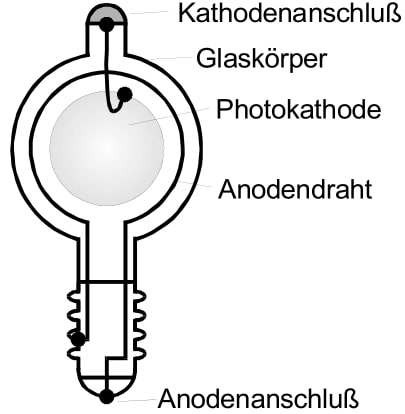
\includegraphics[width=0.5\textwidth]{images/Photozelle.jpg}
        \caption{Diese Grafik zeigt den schematischen Aufbau einer Photozelle \cite{V500}. Zusehen ist der evakuierte Glaskörper, der eine Photokathode samt Anodendraht beinhaltet.}
        \label{fig:1}
    \end{figure}
    \flushleft{Da\;}\justifying die Frequenzen des Lichts unabdingbar für die Messungen sind, muss monochromatisches, weißes Licht in dessen Spektrallinien zerlegt werden. Dies wird mithilfe des folgenden 
    Aufbaus erreicht:
    \begin{figure}[H]
        \centering
        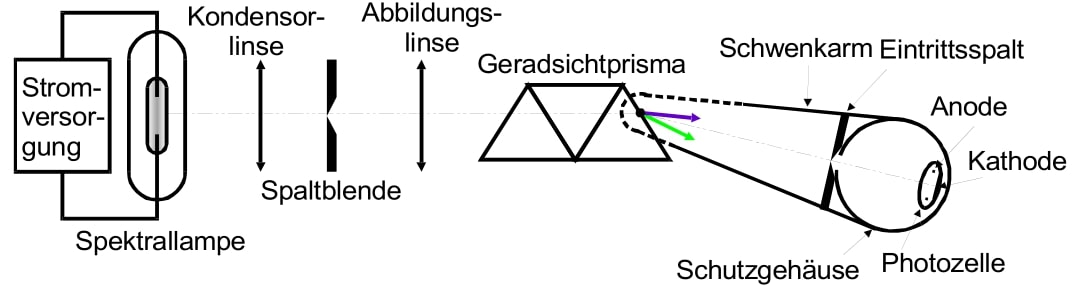
\includegraphics[width=\textwidth]{images/Schema.jpg}
        \caption{Diese Abbildung stellt den schematischen Aufbau der verwendeten Apperatur dar \cite{V500}. Auf der linke Seite befindet sich eine Spektrallampe, welche weißes, monochromatisches
        Licht erzeugt. Dieses Licht wird mithilfe der Kondesorlinse parallel auf die Spaltblende gebündelt. Das Bild des Spalts wird von der Abbildungslinse auf die Photkathode 
        abgebildet und das Geradsichtprisma zerlegt das Licht der Spektrallampe in dessen Spektrallinien.}
        \label{fig:2}
    \end{figure}
    \flushleft{Um\;}\justifying die Energie der losgelösten Elekronen zu bestimmen, wird eine variable Spannung an die Anode und Kathode der Photozelle gelegt. Dieser Strom erzeugt ein Magnetfeld, welches 
    dem Fluss der Elekronen entgegenwirkt. Diese Methode wird Gegenfeldmethode genannt und mit dem folgenden Aufbau durchgeführt:
    \begin{figure}[H]
        \centering
        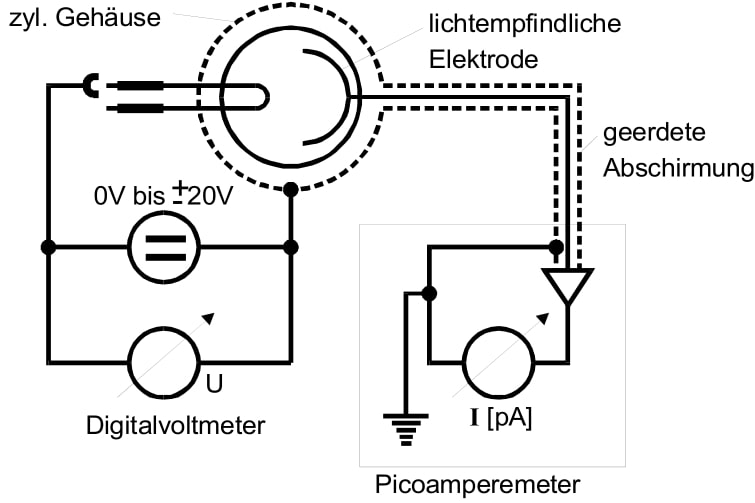
\includegraphics[width=0.75\textwidth]{images/Schaltbild.jpg}
        \caption{Diese Abbildung gibt den schematischen Aufbau der Schaltung der Photozelle wieder \cite{V500}. Mithilfe eines Digitalvoltmeters wird eine Spannung zwischen null und 
        \SI{20}{\volt} angelegt. Diese Spannung erzeugt das Gegenfeld. Das Amperemeter misst den Strom, welcher von den losgelösten Elektronen erzeugt wird.}
        \label{fig:3}
    \end{figure}
    \flushleft{Mithilfe\;}\justifying des Gegenfeldes kann die Energiebilanz aus \eqref{eq:2} erweitert werden, da die kinetische Energie der Elekronen nun gleich der elektrischen Energie $E=e_0 U_g$ sein muss, 
    wobei $e_0$ die Elementarladung und $U_g$ die variable Gegenspannung ist. Daraus ergibt sich die folgende Energiebilanz: \cite{V500}
    \begin{align}
        h\nu &= e_0 U_g + A_k \label{eq:3}
    \end{align}
    \flushleft{Durch\;}\justifying die Einführung eines Gegenfeldes wird erwartet, dass nur die Elektronen mit der größten Geschwinigkeit, also der größten kinetischen Energie, den Anodendraht erreichen. 
    Das bedeutet, dass der Photostrom bei einer bestimmten Gegenspannung augenblicklich verschwindet. Dies würde unter der Annahme auftreten, dass die Elekronen vor der Wechselwirkung
    mit dem Photon gleiche Energie besäßen. Dies ist jedoch nicht der Fall, da Elekronen einen Energieverteilung von 0 bis $\frac{1}{2}m_0 v_{\text{max}}^2$ besitzen. $m_0$ ist 
    hier die Ruhemasse eines Elekrons und $v_{\text{max}}$ die maximale Geschwinigkeit eines ausgelösten Elekrons. Folglich fällt der Photostrom nicht abrupt ab, sondern allmählich.
    Dieses Phänomen wird von der Fermi-Dirac-Statistik veranschaulicht: \cite{V500}
    \begin{figure}[H]
        \centering
        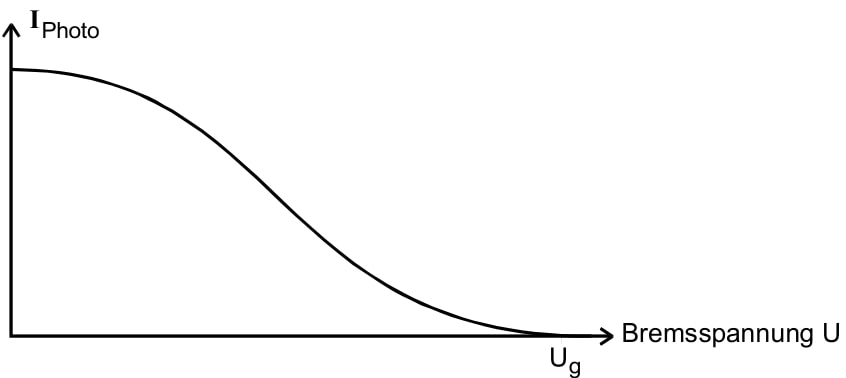
\includegraphics[width=\textwidth]{images/Dirac.jpg}
        \caption{Diese Statistik zeigt den stetigen Verlauf der Abklingkurve des Photostroms $I_{\text{Photo}}$ gegenüber der Bremsspannung $U$ \cite{V500}.}
        \label{fig:4}
    \end{figure}
    \flushleft{Da\;}\justifying nicht vorrausgesetzt werden kann, dass alle emittierten Photonen die Photokathode erreichen, ist die Fermi-Dirac-Statistik nicht aussagekräftig genug, 
    um die Gegenspannung $U_g$ zweifelsfrei zu bestimmen. Deshalb wird die parabolische Beziehung zwischen Photostrom und Bremsspannung \cite{V500}
    \begin{align}
        I_{\text{Photo}} &\propto U^2 \Leftrightarrow \sqrt{I_{\text{Photo}}} \propto U \label{eq:4}
    \end{align}
    \flushleft{verwendet,\;}\justifying um über den Schnittpunkt der entstehenden Geraden mit der x-Achse die Gegenspannung $U_g$ zu erhalten.

\newpage
\section{Versuchsaufbau und Durchführung}

    \flushleft{Für\;}\justifying diesen Versuch wird der folgende Aufbau verwendet:
    \begin{figure}[H]
        \centering
        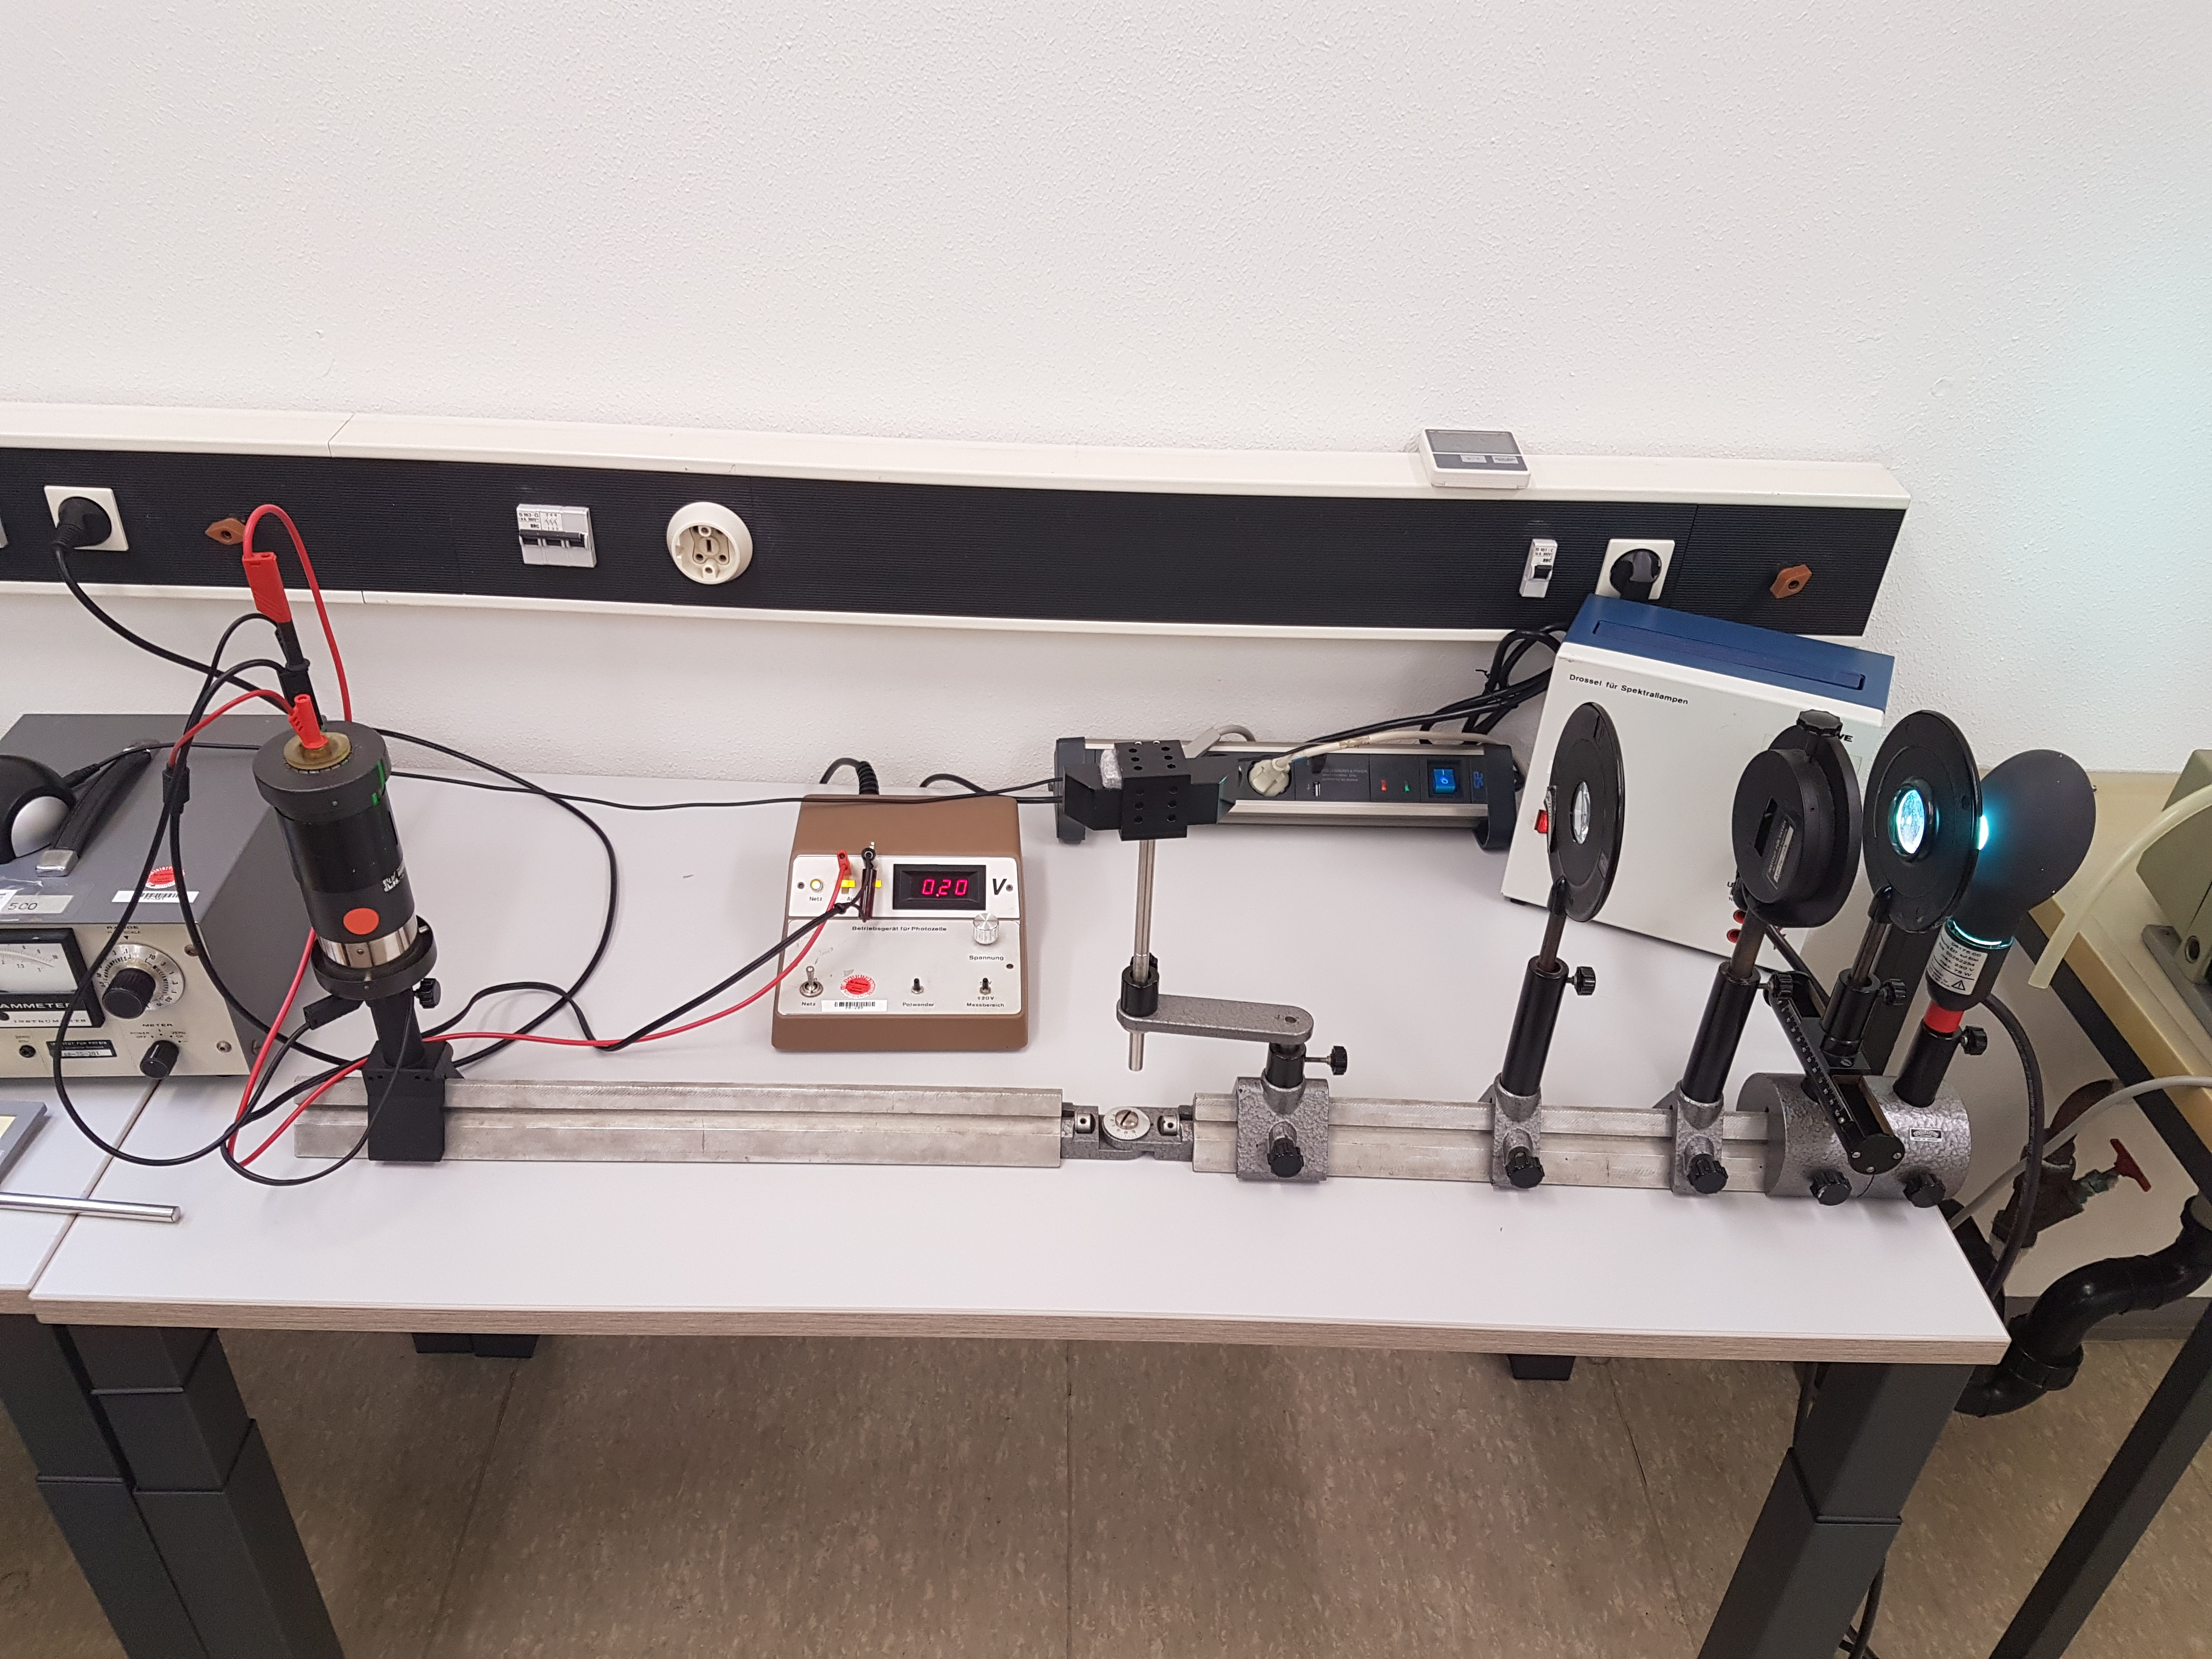
\includegraphics[width=\textwidth]{images/Aufbau.jpg}
        \caption{In dieser Abbildung ist der verwendete Versuchsaufbau zu sehen. Dieser ähnelt dem schematischen Aufbau aus Abbildung \ref{fig:2}. Hier ist die Photozelle
        auf der linken Seite. In der mitte befindet sich das Geradsichtprisma, welches über einen Schwenkarm auf der Stativschiene befestigt ist. Rechts daneben befindet 
        sich die Abbildungslinse, gefolgt von der Spaltblende. Zwischen Blende und Spektrallampe befindet sich die Kondesorlinse. An der Photozelle ist ein Digitalvoltmeter
        und ein Amperemeter angeschlossen.}
        \label{fig:5}
    \end{figure}
    \flushleft{An\;}\justifying die Photozelle werden ein Digitalvoltmeters und Amperemeter angeschlossen, mit welchen Bremsspannung und Photostrom eingestellt, beziehungsweise 
    abgelesen werden. Die hier verwendete Spektrallampe ist eine Quecksilberlampe, welche die folgenden primären Spektrallinien produziert:
    \begin{figure}[H]
        \centering
        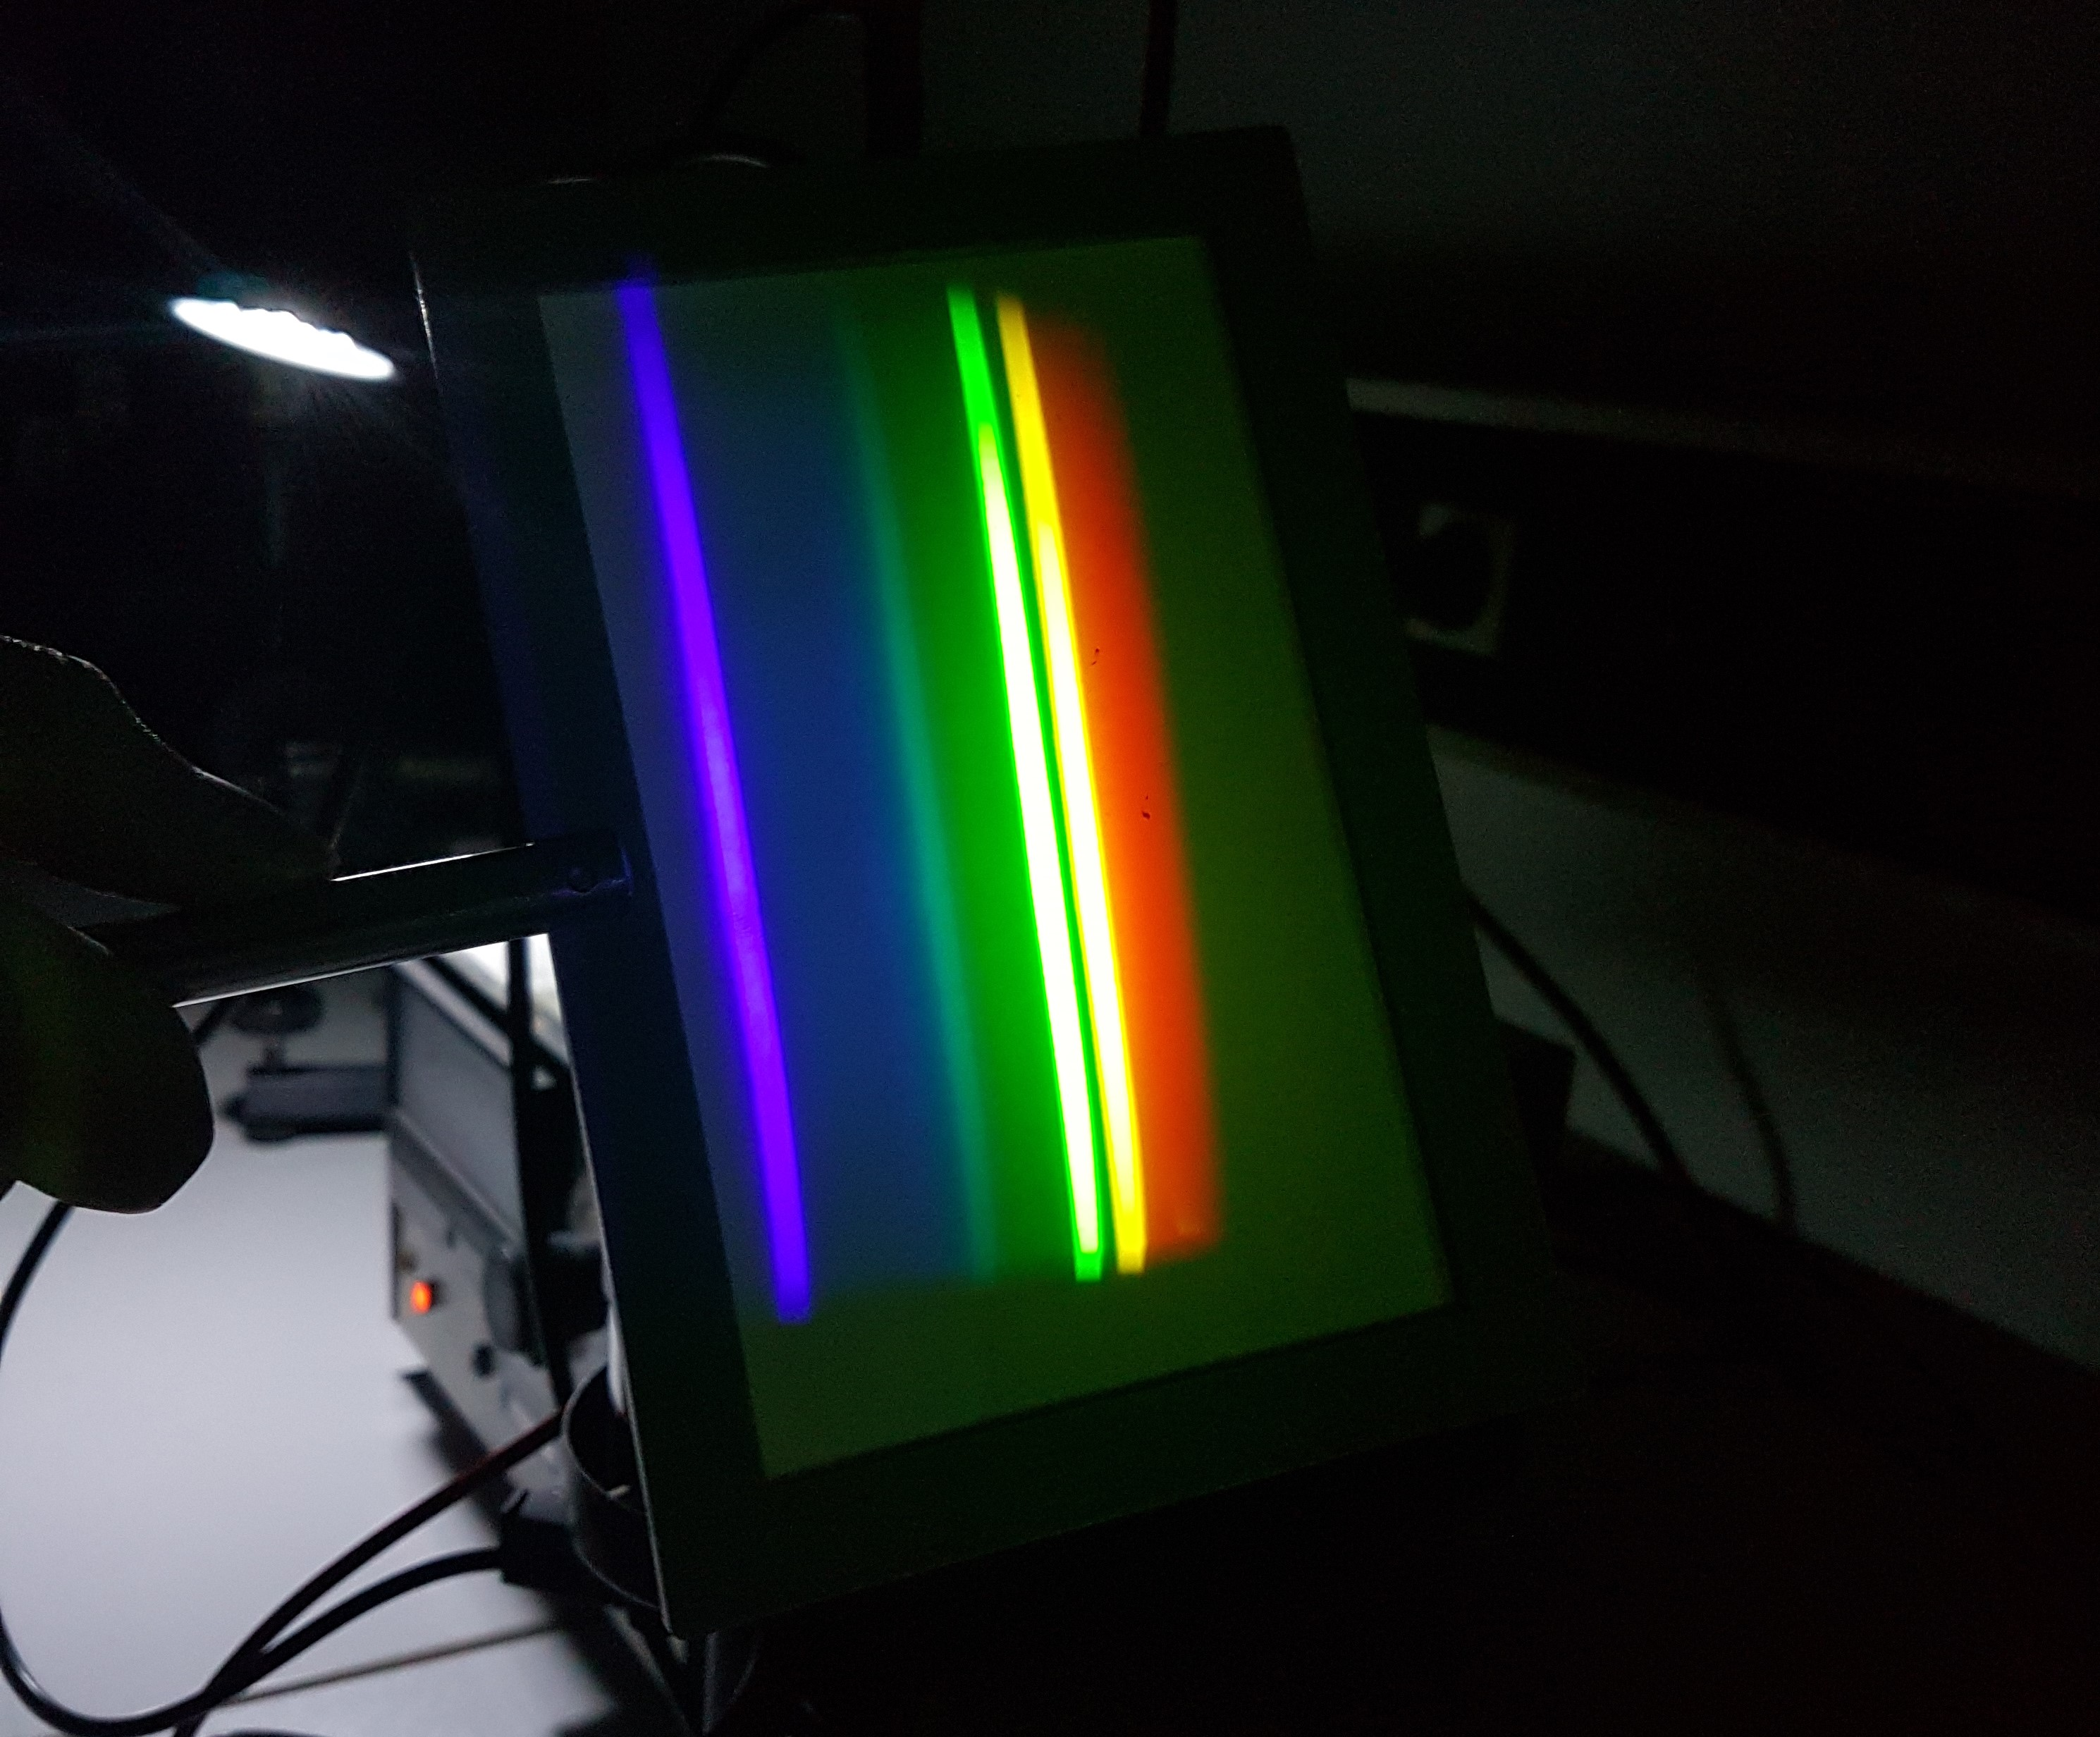
\includegraphics[width=0.5\textwidth]{images/Spektral.jpg}
        \caption{Hier ist das Spektralmuster der Quecksilberlampe zu erkennen. Deutlich zu erkennen sind die Linien violett, grün und gelb. Die in diesem Versuch gemessenen 
        Linien sind grün, gelb und rot.}
        \label{fig:6}
    \end{figure}
    \flushleft{Für\;}\justifying die gelbe Spektrallinie werden 27 Messwerte aufgenommen. Die Spannung wird in \SI{1}{\volt}-Schritten in einem Intervall von 
    \SI{18.96}{\volt} $\leq$ U $\leq$ \SI{0.02}{\volt} variiert . Dabei wird der jeweilige Photostrom dem Amperemeter entnommen. Zwischen \SI{7}{\volt} $\leq$ U $\leq$ \SI{0.5}{\volt}
    wird der Strom in \SI{0.5}{\volt}-Schritten abgelesen.
    Bei den Spektrallinien rot und grün werden je zehn Messwerte in \SI{0.2}{\volt}-Schritten aufgenommen in dem Intervall \SI{2}{\volt} $\leq$ U $\leq$ \SI{0.2}{\volt}. 

\section{Auswertung}

    \begin{figure}[H]
        \centering
        \includegraphics[width=0.5\textwidth]{build/plotGelb.pdf}
        \caption{Gelb}
        \label{fig:7}
    \end{figure}

    \begin{figure}[H]
        \centering
        \includegraphics[width=0.5\textwidth]{build/plotGruen.pdf}
        \caption{Grün}
        \label{fig:8}
    \end{figure}

    \begin{figure}[H]
        \centering
        \includegraphics[width=0.5\textwidth]{build/plotRot.pdf}
        \caption{Rot}
        \label{fig:9}
    \end{figure}

\section{Diskussion}

\newpage
\printbibliography

\newpage
\section{Appendix}

\begin{table}[H]
    \centering
    \caption{}
    \input{Gelb.tex}
    \label{tab:1}
\end{table}

\begin{table}[H]
    \centering
    \caption{}
    \input{Gruen.tex}
    \label{tab:2}
\end{table}

\begin{table}[H]
    \centering
    \caption{}
    \input{Rot.tex}
    \label{tab:3}
\end{table}

\end{document}


